\documentclass[10pt]{beamer}

\newcommand{\lectnum}{L03}
\newcommand{\lecttitle}{Linear Regression and Classification: Part II}

\usepackage{amsmath, amssymb, graphicx}
\usepackage[]{algorithm2e}
\usepackage{pdfpages}
\usepackage{bm}
\usepackage{relsize}
\usepackage[british]{babel}
\usepackage{tikz,tikzsymbols}
\usepackage{pgfplots}
\pgfplotsset{compat=1.17}
\usepackage{hyperref}
\usepackage{cancel}
\usepackage{caption,subcaption}
\usepackage{adjustbox}
\usepackage{overpic}
\usepackage[UKenglish]{isodate}

\usetikzlibrary{arrows,decorations.markings,positioning}

\newcommand{\bs}{\boldsymbol}


\hypersetup{colorlinks,linkcolor=,urlcolor=blue}
\newenvironment{titledslide}[1]{\begin{frame}\frametitle{#1}}{\end{frame}}

\mode<presentation>{\setbeamercovered{transparent}}

\setbeamertemplate{sidebar right}{}
\setbeamertemplate{footline}{%
\hfill\usebeamertemplate***{navigation symbols}
\hspace{0.4cm}\lectnum: \insertframenumber{}/\inserttotalframenumber \hspace*{0.4cm}}

\author{Mengyan Zhang}

\title{COMS20018, Introduction to AI:\\ \vspace{5pt} \lecttitle}

\institute{School of Computer Science\\University of Bristol}
\date{28th September 2026}

%%%%%%%%%%%%%%%%%%%%%%%%%%%%%%%%%%%%%%%%%%%%%%%%%%%%%%%%%%%%%%%%%%%%%%

\begin{document}
%%%%%%%%%%%%%%%%%%%%%%%%%%%%%%%%%%%%%%%%%%%%%%%%%%%%%%%%%%%%%%%%%%%%%%

\begin{frame}[fragile]
  \begin{tikzpicture}[remember picture, overlay]
    \node[anchor=north west, xshift=0.4cm, yshift=-0.4cm] at (current page.north west)
      {
\includegraphics[width=3.4cm]{figures/uob_logo.png}};
  \end{tikzpicture}
  \titlepage
\end{frame}
%%%%%%%%%%%%%%%%%%%%%%%%%%%%%%%%%%%%%%%%%%%%%%%%%%%%%%%%%%%%%%%%%%%%%%
\begin{frame}[fragile]

  \frametitle{Agenda}
  \begin{itemize}
  \item Linear regression: recap and extensions \hfill
    \begin{itemize}
    \item Recap: least squares
    \item High-dimensional inputs
    \item A probabilistic view: maximum likelihood
    \end{itemize}
  \item Overfitting \hfill
    \begin{itemize}
    \item Choosing $M$: under/overfitting
    \item Regularized least squares
    \end{itemize}
  \item Linear classification \hfill
    \begin{itemize}
    \item Logistic regression \& the decision boundary
    \item Fitting with the cross-entropy loss
    \item Evaluation metrics
    \end{itemize}
  \item A general view: loss functions
  \item Optimisation \hfill
    \begin{itemize}
    \item Gradient descent \& stochastic gradient descent (SGD)
    \end{itemize}
  \end{itemize}

\end{frame}
%%%%%%%%%%%%%%%%%%%%%%%%%%%%%%%%%%%%%%%%%%%%%%%%%%%%%%%%%%%%%%%%%%%%%%
\begin{frame}[fragile]
\frametitle{Recap: linear regression \& least squares}

\begin{columns}[T]
\begin{column}{0.4\textwidth}
\centerline{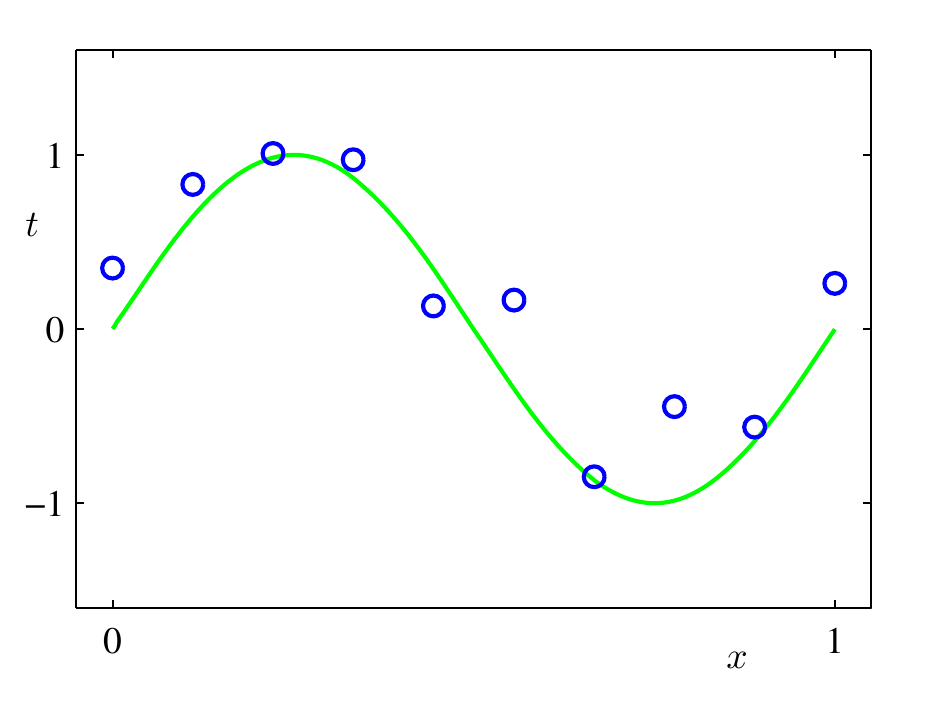
\includegraphics[width=\textwidth]{figures/prml_fig1_2.png}}

\vspace{4pt}
{\scriptsize Bishop, \emph{PRML} (2006), Fig.\ 1.2: $N{=}10$ points
sampled from $\sin(2\pi x)$ plus random noise.}
\end{column}
\begin{column}{0.57\textwidth}
\begin{itemize}
\item \textbf{Problem}: given data $\{(x_n,t_n)\}_{n=1}^N$, learn
  $y(x,\bs{w}) = \bs{w}^\top\bs\phi(x)$ to predict $t$ for a new $x$.
\item \textbf{Least squares}: choose $\bs{w}$ to minimise the
  sum-of-squares loss
\[
L_D(\bs{w}) = \frac12\sum_{n=1}^N \bigl\{t_n - y(x_n,\bs{w})\bigr\}^2
\]
\end{itemize}
\end{column}
\end{columns}

\vspace{6pt}
\begin{itemize}
\item \textbf{Closed-form solution} (the normal equations): with design
  matrix $\Phi_{nj} = \phi_j(x_n)$ and targets $\bs{t} =
  (t_1,\dots,t_N)^\top$,
\[
\bs{w}_{\mathrm{ML}} = \bigl(\Phi^\top \Phi\bigr)^{-1} \Phi^\top \bs{t} =
\Phi^\dagger \bs{t}
\]
where $\Phi^\dagger$ is the (Moore-Penrose) \textbf{pseudo-inverse} of
$\Phi$.
\item[$\Rightarrow$] See L02 for the full derivation and a worked
  example.
\end{itemize}

\end{frame}
%%%%%%%%%%%%%%%%%%%%%%%%%%%%%%%%%%%%%%%%%%%%%%%%%%%%%%%%%%%%%%%%%%%%%%
\begin{frame}[fragile]
\frametitle{High-dimensional inputs}

\begin{itemize}
\item In practice the input is a \textbf{vector}, $\bs{x} =
  (x_1,\dots,x_D)^\top \in \mathbb{R}^D$, e.g.\ a house's size, rooms,
  age, distance to centre.
\item Linear basis function model (Bishop eq.\ 3.2), with
  $\phi_0(\bs{x}) = 1$:
\[
y(\bs{x},\bs{w}) = w_0 + \sum_{j=1}^{M-1} w_j\,\phi_j(\bs{x})
= \bs{w}^\top\bs\phi(\bs{x})
\]
  % \begin{itemize}
  % \item \textbf{Linear}: $\phi_j(\bs{x}) = x_j$ $\Rightarrow$
  %   $y = w_0 + \sum_{j=1}^{D} w_j x_j$ (multiple linear regression,
  %   $M{=}D{+}1$)
  % \item \textbf{Nonlinear}: e.g.\ Gaussians $\phi_j(\bs{x}) =
  %   \exp\{-\|\bs{x}-\bs\mu_j\|^2/2s^2\}$, or products such as $x_1x_2$,
  %   $x_1^2$, \dots
  % \end{itemize}
\item Design matrix $\Phi_{nj} = \phi_j(\bs{x}_n)$ is still $N\times M$,
  so $\bs{w}_{\mathrm{ML}} = \Phi^\dagger\bs{t}$ is \emph{unchanged}.
% \item[$\Rightarrow$] Caution: a full cubic polynomial in $D$ variables
  % already has $\sim D^3$ terms (the \emph{curse of dimensionality}).
\item Targets can be vectors too, $\bs{t}_n\in\mathbb{R}^K$; in this
  lecture we keep $t$ \textbf{scalar}.
\end{itemize}

% \vspace{2pt}
% \begin{itemize}
% \item[$\Rightarrow$] From now on we write $\bs{x}$; our running
%   $\sin(2\pi x)$ example is simply the case $D{=}1$.
% \end{itemize}

\vspace{2pt}
{\scriptsize See Bishop, \emph{PRML} (2006), Sections 1.4 and 3.1.}

\end{frame}
%%%%%%%%%%%%%%%%%%%%%%%%%%%%%%%%%%%%%%%%%%%%%%%%%%%%%%%%%%%%%%%%%%%%%%
\begin{frame}[fragile]
\frametitle{A probabilistic view: maximum likelihood}

\begin{itemize}
\item Assume the target is the model prediction plus \textbf{Gaussian
  noise}:
\[
t = y(\bs{x},\bs{w}) + \varepsilon, \qquad \varepsilon \sim \mathcal{N}(0,\beta^{-1})
\]
where $\beta$ is the noise \textbf{precision} (inverse variance).
\item Equivalently: $p(t\mid \bs{x},\bs{w},\beta) = \mathcal{N}\bigl(t \mid
y(\bs{x},\bs{w}),\, \beta^{-1}\bigr)$.
\end{itemize}

\begin{itemize}
\item For independent and identically distributed (i.i.d.)\ data
  $\{\bs{x}_n, t_n\}_{n=1}^N$, the \textbf{likelihood} is the product
\[
p(\bs{t}\mid \bs{w},\beta) = \prod_{n=1}^{N} \mathcal{N}\bigl(t_n \mid
y(\bs{x}_n,\bs{w}),\, \beta^{-1}\bigr)
\]
\item[$\Rightarrow$] Likelihood tells us how well a particular choice of
  model parameters explains the observed data.
\item[$\Rightarrow$] High likelihood: observed $t_n$ are close to what
  the model predicts.
\end{itemize}

\end{frame}
%%%%%%%%%%%%%%%%%%%%%%%%%%%%%%%%%%%%%%%%%%%%%%%%%%%%%%%%%%%%%%%%%%%%%%
\begin{frame}[fragile]
\frametitle{Maximum likelihood: the log-likelihood}

\begin{itemize}
\item Recall the likelihood:
\[
p(\bs{t}\mid \bs{w},\beta) = \prod_{n=1}^{N} \mathcal{N}\bigl(t_n \mid
y(\bs{x}_n,\bs{w}),\, \beta^{-1}\bigr)
\]
\item Taking $\ln$ turns the product into a sum, the
  \textbf{log-likelihood}:
\[
\ln p(\bs{t}\mid \bs{w},\beta) = -\beta\, L_D(\bs{w}) + \frac{N}{2}\ln\beta -
\frac{N}{2}\ln(2\pi)
\]
\item[$\Rightarrow$] Maximising this over $\bs{w}$ (for fixed $\beta$) is
  \emph{exactly the same} as minimising $L_D(\bs{w})$: $\bs{w}_{\mathrm{ML}}$
  is identical to the least-squares solution from last lecture.
\end{itemize}

\end{frame}
%%%%%%%%%%%%%%%%%%%%%%%%%%%%%%%%%%%%%%%%%%%%%%%%%%%%%%%%%%%%%%%%%%%%%%
\begin{frame}[fragile]
\frametitle{Maximum likelihood: what we get for free}

\begin{itemize}
\item Least squares only ever gave us a point prediction $y(\bs{x},\bs{w})$.
\item The probabilistic view also gives us the \textbf{noise level}: setting
  $\partial \ln p / \partial \beta = 0$,
\[
\frac{1}{\beta_{\mathrm{ML}}} = \frac{1}{N}\sum_{n=1}^{N} \bigl\{t_n -
y(\bs{x}_n,\bs{w}_{\mathrm{ML}})\bigr\}^2
\]
i.e.\ the residual variance.
\end{itemize}

\begin{columns}[T]
\begin{column}{0.45\textwidth}
\centerline{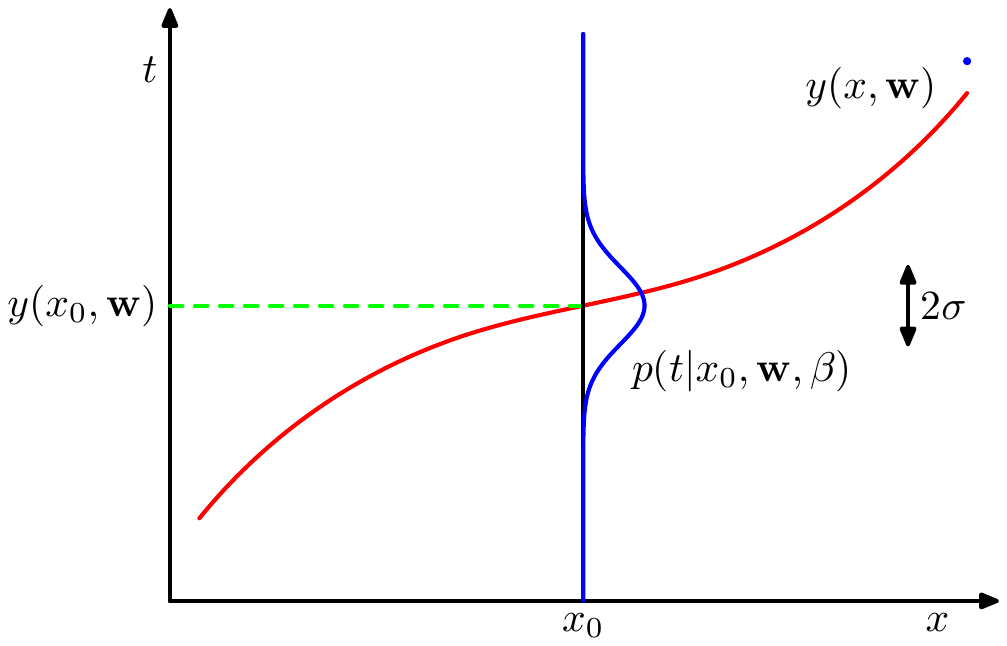
\includegraphics[width=\textwidth]{figures/prml_fig1_16.png}}

\vspace{2pt}
{\scriptsize Bishop, \emph{PRML} (2006), Fig.\ 1.16: at a new input
$x_0$, a Gaussian over $t$ centred on $y(x_0,\bs{w})$, with
$\beta^{-1} = \sigma^2$.}
\end{column}
\begin{column}{0.52\textwidth}
\begin{itemize}
\item[$\Rightarrow$] Now we can report a full predictive
  \emph{distribution} $p(t\mid \bs{x},\bs{w}_{\mathrm{ML}},\beta_{\mathrm{ML}})$,
  not just a single number, e.g.\ ``$\pm$ how much'' around each
  prediction.
\end{itemize}
\end{column}
\end{columns}

\end{frame}
%%%%%%%%%%%%%%%%%%%%%%%%%%%%%%%%%%%%%%%%%%%%%%%%%%%%%%%%%%%%%%%%%%%%%%
\begin{frame}[fragile]
\frametitle{Overfitting vs.\ underfitting: choosing $M$}

\centerline{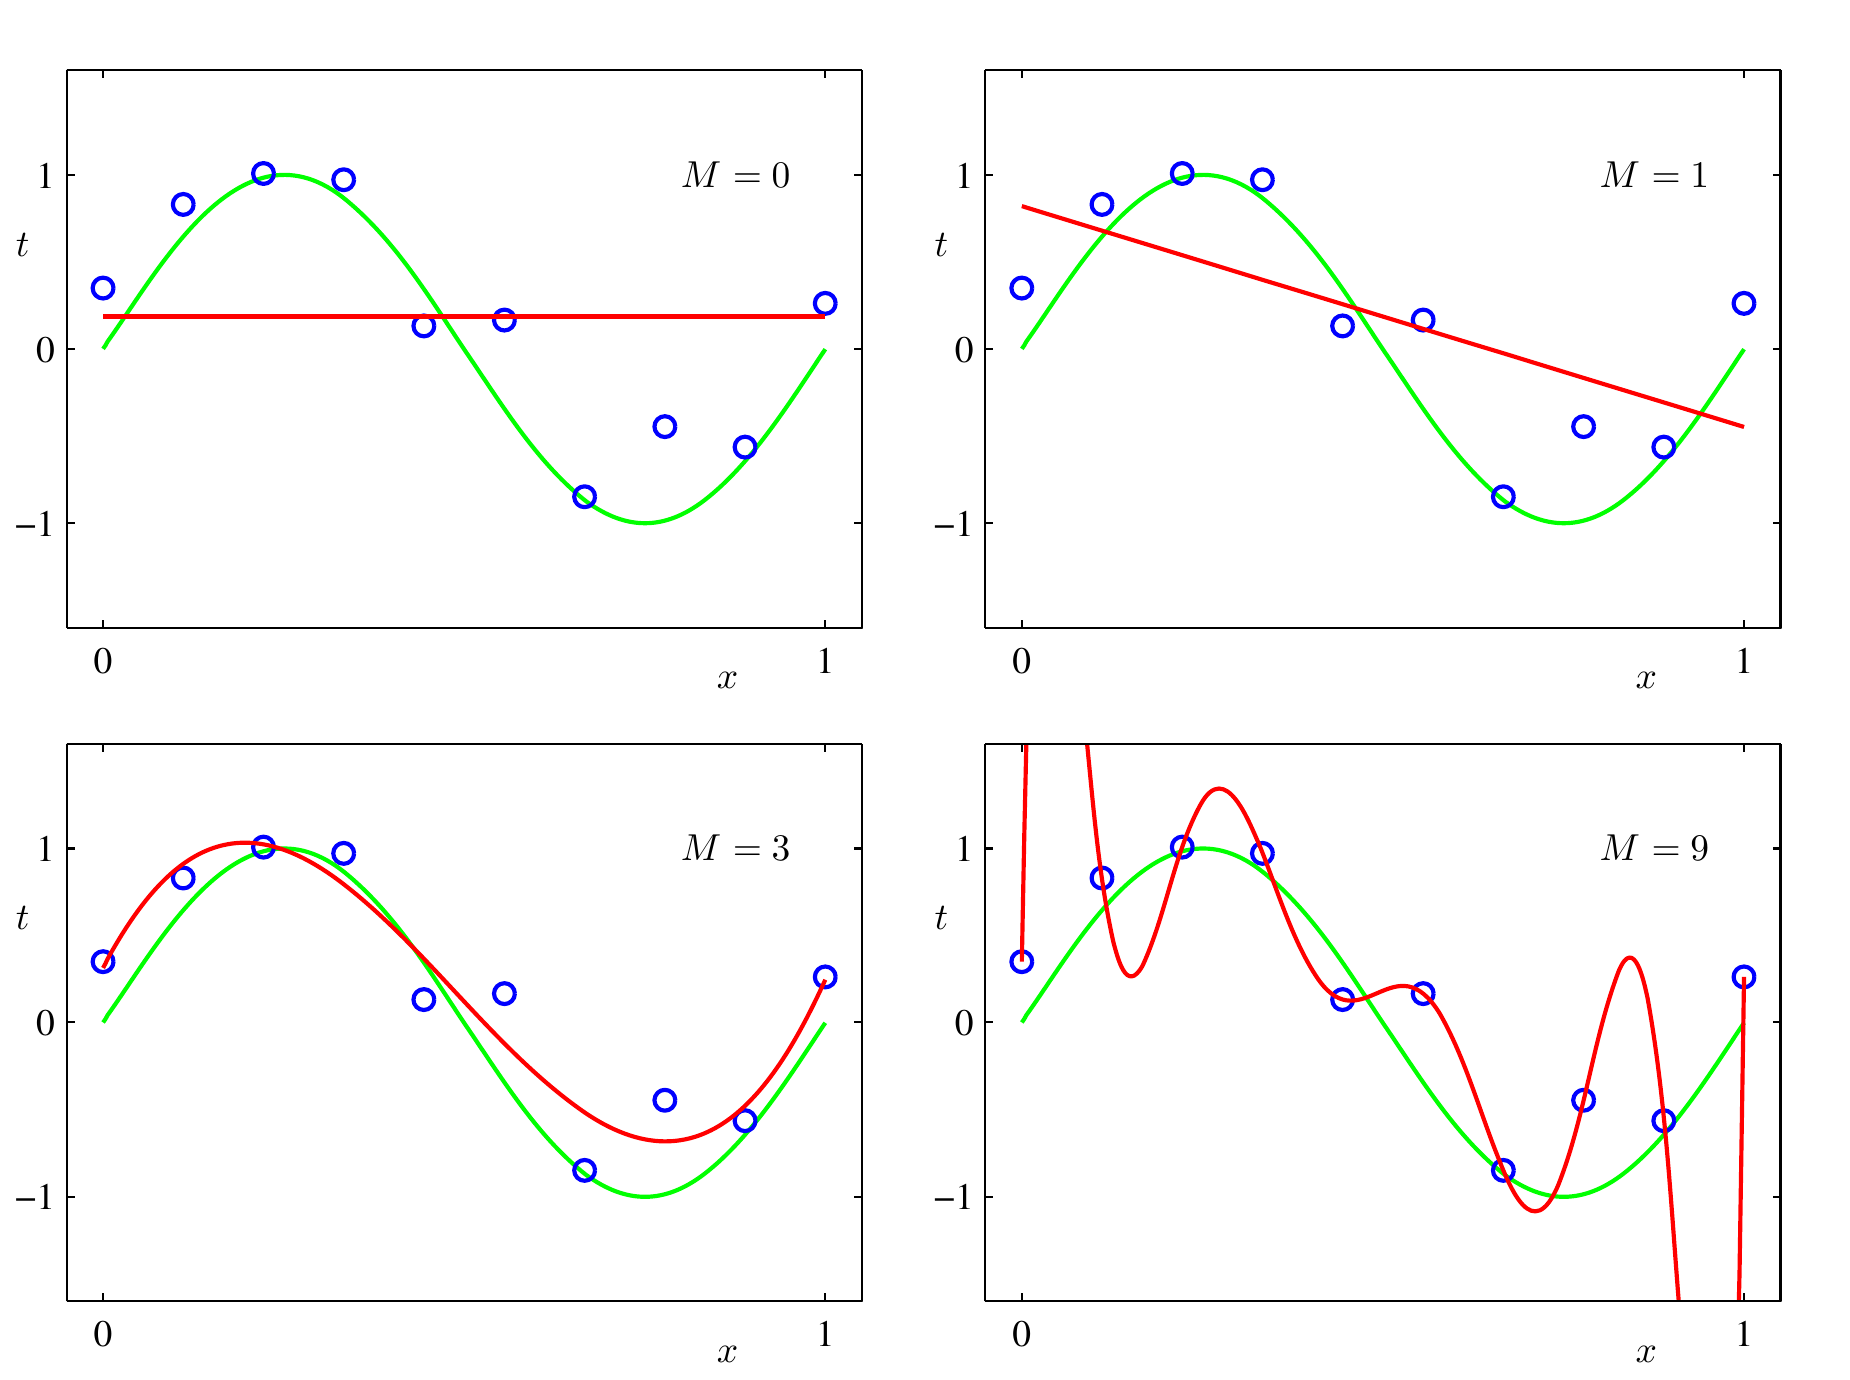
\includegraphics[width=0.62\textwidth]{figures/prml_fig1_4.png}}

\vspace{2pt}
{\scriptsize Bishop, \emph{PRML} (2006), Fig.\ 1.4: least-squares fits
(red) of order $M=0,1,3,9$ to the data from Fig.\ 1.2 (green =
true $\sin(2\pi x)$).}

\vspace{4pt}
\begin{itemize}
\item $M{=}0,1$: too rigid, \textbf{underfit}, miss the curve's shape.
\item $M{=}3$: about right, close to $\sin(2\pi x)$.
\item $M{=}9$: passes through \emph{every} data point exactly
  ($L_D(\bs{w}^\star)=0$) but oscillates wildly, \textbf{overfits}.
\end{itemize}

\end{frame}
%%%%%%%%%%%%%%%%%%%%%%%%%%%%%%%%%%%%%%%%%%%%%%%%%%%%%%%%%%%%%%%%%%%%%%
\begin{frame}[fragile]
\frametitle{Overfitting vs.\ underfitting: choosing $M$}

\centerline{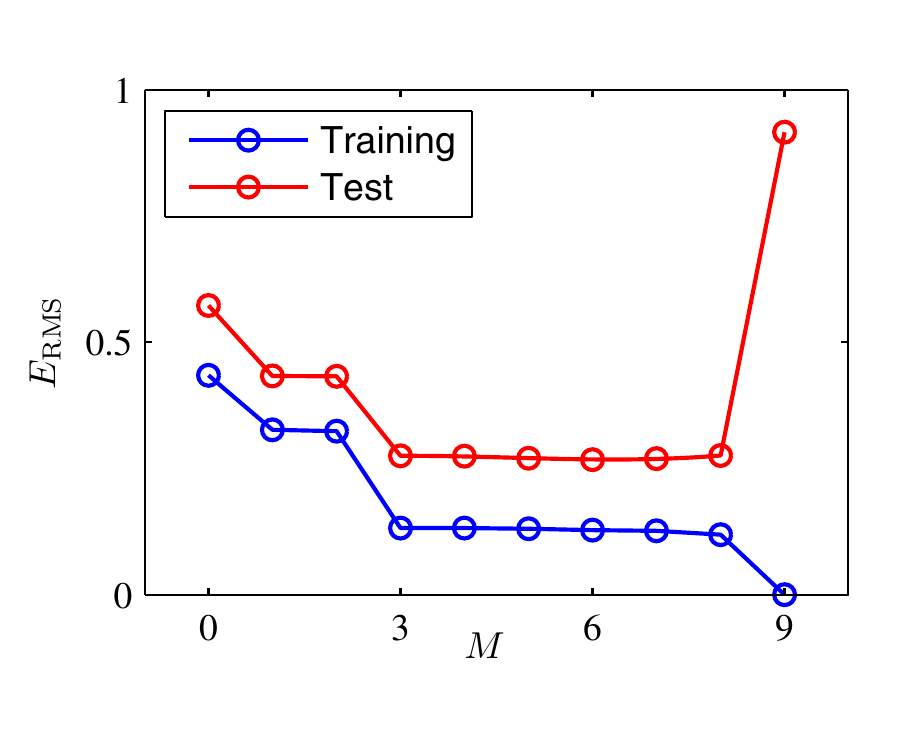
\includegraphics[width=0.48\textwidth]{figures/prml_fig1_5.png}}

\vspace{2pt}
{\scriptsize Bishop, \emph{PRML} (2006), Fig.\ 1.5: root-mean-square
error $E_{\mathrm{RMS}} = \sqrt{2L_D(\bs{w}^\star)/N}$ on the training
set vs.\ a held-out test set, for each $M$.}

\vspace{4pt}
\begin{itemize}
\item Training error falls monotonically with $M$; more parameters
  can only fit the training data better (or equally well).
\item Test error is \textbf{U-shaped}: too low $M$ underfits, too high
  $M$ overfits; here $M{=}3$--$8$ generalises best.
% \item[$\Rightarrow$] Least squares (recap above) and regularization
  % (later today) are both, in some form, about getting this choice
  % right.
\end{itemize}

\end{frame}
%%%%%%%%%%%%%%%%%%%%%%%%%%%%%%%%%%%%%%%%%%%%%%%%%%%%%%%%%%%%%%%%%%%%%%
\begin{frame}[fragile]
\frametitle{Why regularize? Overfitting shows up as huge weights}

\begin{columns}[T]
\begin{column}{0.5\textwidth}
\newcommand{\R}[1]{\textcolor{red!70!black}{#1}}
\resizebox{\columnwidth}{!}{%
\begin{tabular}{c|rrrr}
 & $M{=}0$ & $M{=}1$ & $M{=}3$ & \R{$M{=}9$}\\ \hline
$w_0^\star$ & 0.19 & 0.82 & 0.31 & \R{0.35}\\
$w_1^\star$ &  & $-1.27$ & 7.99 & \R{232.37}\\
$w_2^\star$ &  &  & $-25.43$ & \R{$-5321.83$}\\
$w_3^\star$ &  &  & 17.37 & \R{48568.31}\\
$w_4^\star$ &  &  &  & \R{$-231639.30$}\\
$w_5^\star$ &  &  &  & \R{640042.26}\\
$w_6^\star$ &  &  &  & \R{$-1061800.52$}\\
$w_7^\star$ &  &  &  & \R{1042400.18}\\
$w_8^\star$ &  &  &  & \R{$-557682.99$}\\
$w_9^\star$ &  &  &  & \R{125201.43}
\end{tabular}}

\vspace{4pt}
{\scriptsize Bishop, \emph{PRML} (2006), Table 1.1: least-squares
coefficients for the polynomial fits in Fig.\ 1.4.}
\end{column}
\begin{column}{0.47\textwidth}
\begin{itemize}
\item As $M$ grows, the magnitude of the fitted coefficients
  \textbf{blows up}.
\item $M{=}9$: huge positive and negative weights, finely tuned to
  cancel exactly at the $N{=}10$ data points, hence the wild
  oscillations in between.
\item[$\Rightarrow$] Idea: keep the flexible model, but
  \textbf{discourage large weights}.
\end{itemize}
\end{column}
\end{columns}

\end{frame}
%%%%%%%%%%%%%%%%%%%%%%%%%%%%%%%%%%%%%%%%%%%%%%%%%%%%%%%%%%%%%%%%%%%%%%
\begin{frame}[fragile]
\frametitle{Regularized least squares}

\begin{itemize}
\item Penalise large weights. Add a \textcolor{orange!85!black}{regularization term} to the
  loss:
\[
L(\bs{w}) = L_D(\bs{w}) + \textcolor{orange!85!black}{\lambda\, L_W(\bs{w})}, \qquad
\textcolor{orange!85!black}{L_W(\bs{w}) = \frac{1}{2}\bs{w}^\top\bs{w}}
\]
($\lambda$ = regularization coefficient). This is \textbf{ridge regression}.
\end{itemize}

\begin{itemize}
\item Still quadratic in $\bs{w}$ $\Rightarrow$ still closed-form:
\[
\bs{w} = \bigl(\textcolor{orange!85!black}{\lambda \mathbf{I}} + \Phi^\top\Phi\bigr)^{-1}\Phi^\top\bs{t}
\]
\item $\lambda{=}0$: back to plain least squares. $\lambda \to \infty$:
  $\bs{w}\to \mathbf{0}$, controls model complexity \emph{without}
  changing $M$.
\end{itemize}

\begin{itemize}
\item[$\Rightarrow$] More general penalty $\textcolor{orange!85!black}{\sum_j |w_j|^q}$: $q{=}2$ is ridge
  above; $q{=}1$ (\textbf{lasso}) additionally drives many $w_j$ exactly to
  zero, automatic feature selection.
\end{itemize}

\end{frame}
%%%%%%%%%%%%%%%%%%%%%%%%%%%%%%%%%%%%%%%%%%%%%%%%%%%%%%%%%%%%%%%%%%%%%%
\begin{frame}[fragile]
\frametitle{Discuss: how can we reduce overfitting?}
\setbeamertemplate{blocks}[rounded]
\setbeamercolor{block title}{bg=orange!25,fg=black}
\setbeamercolor{block body}{bg=orange!7,fg=black}


\begin{block}{Discuss with your neighbour (1 min)}
Our $M{=}9$ polynomial overfits. List as many ways as you can to stop a
model overfitting.
\end{block}

\vspace{6pt}
\visible<2->{%
\begin{itemize}
\item \textbf{More training data}: for a fixed $M$, overfitting shrinks
  as $N$ grows
\item \textbf{Simpler model}: choose $M$ (or fewer features) using a
  validation set or cross-validation
\item \textbf{Regularization}: penalise large weights, e.g.\ ridge
  ($q{=}2$) or lasso ($q{=}1$); tune $\lambda$ on validation data
\item \textbf{For neural networks} (L04 onwards): early stopping,
  dropout, data augmentation
\item[$\Rightarrow$] All trade fit to the training data against how
  well the model generalises; always judge on held-out data.
\end{itemize}}

\end{frame}
%%%%%%%%%%%%%%%%%%%%%%%%%%%%%%%%%%%%%%%%%%%%%%%%%%%%%%%%%%%%%%%%%%%%%%
\begin{frame}[fragile]
\frametitle{From regression to classification}

\begin{itemize}
\item So far: target $t \in \mathbb{R}$ (continuous). Now: assign
  $\bs{x}$ to one of $K$ discrete \textbf{classes} $C_1,\dots,C_K$.
\item Two classes ($K{=}2$): a single scalar $t\in\{0,1\}$ suffices,
  with $t{=}1$ for $C_1$ and $t{=}0$ for $C_2$.
\item General case, \textbf{1-of-$K$} (one-hot) coding: $\bs{t} \in
  \{0,1\}^K$ with a single 1 marking the class, e.g.\ for $K{=}5$ and
  class $C_2$,
\[
\bs{t} = (0,1,0,0,0)^\top
\]
\item[$\Rightarrow$] Today we focus on $K{=}2$; see Bishop \S4.3.4 for
  the multiclass details.
\end{itemize}


\end{frame}
%%%%%%%%%%%%%%%%%%%%%%%%%%%%%%%%%%%%%%%%%%%%%%%%%%%%%%%%%%%%%%%%%%%%%%
\begin{frame}[fragile]
\frametitle{Classification in practice}

\begin{columns}[b]
\begin{column}{0.48\textwidth}
\centerline{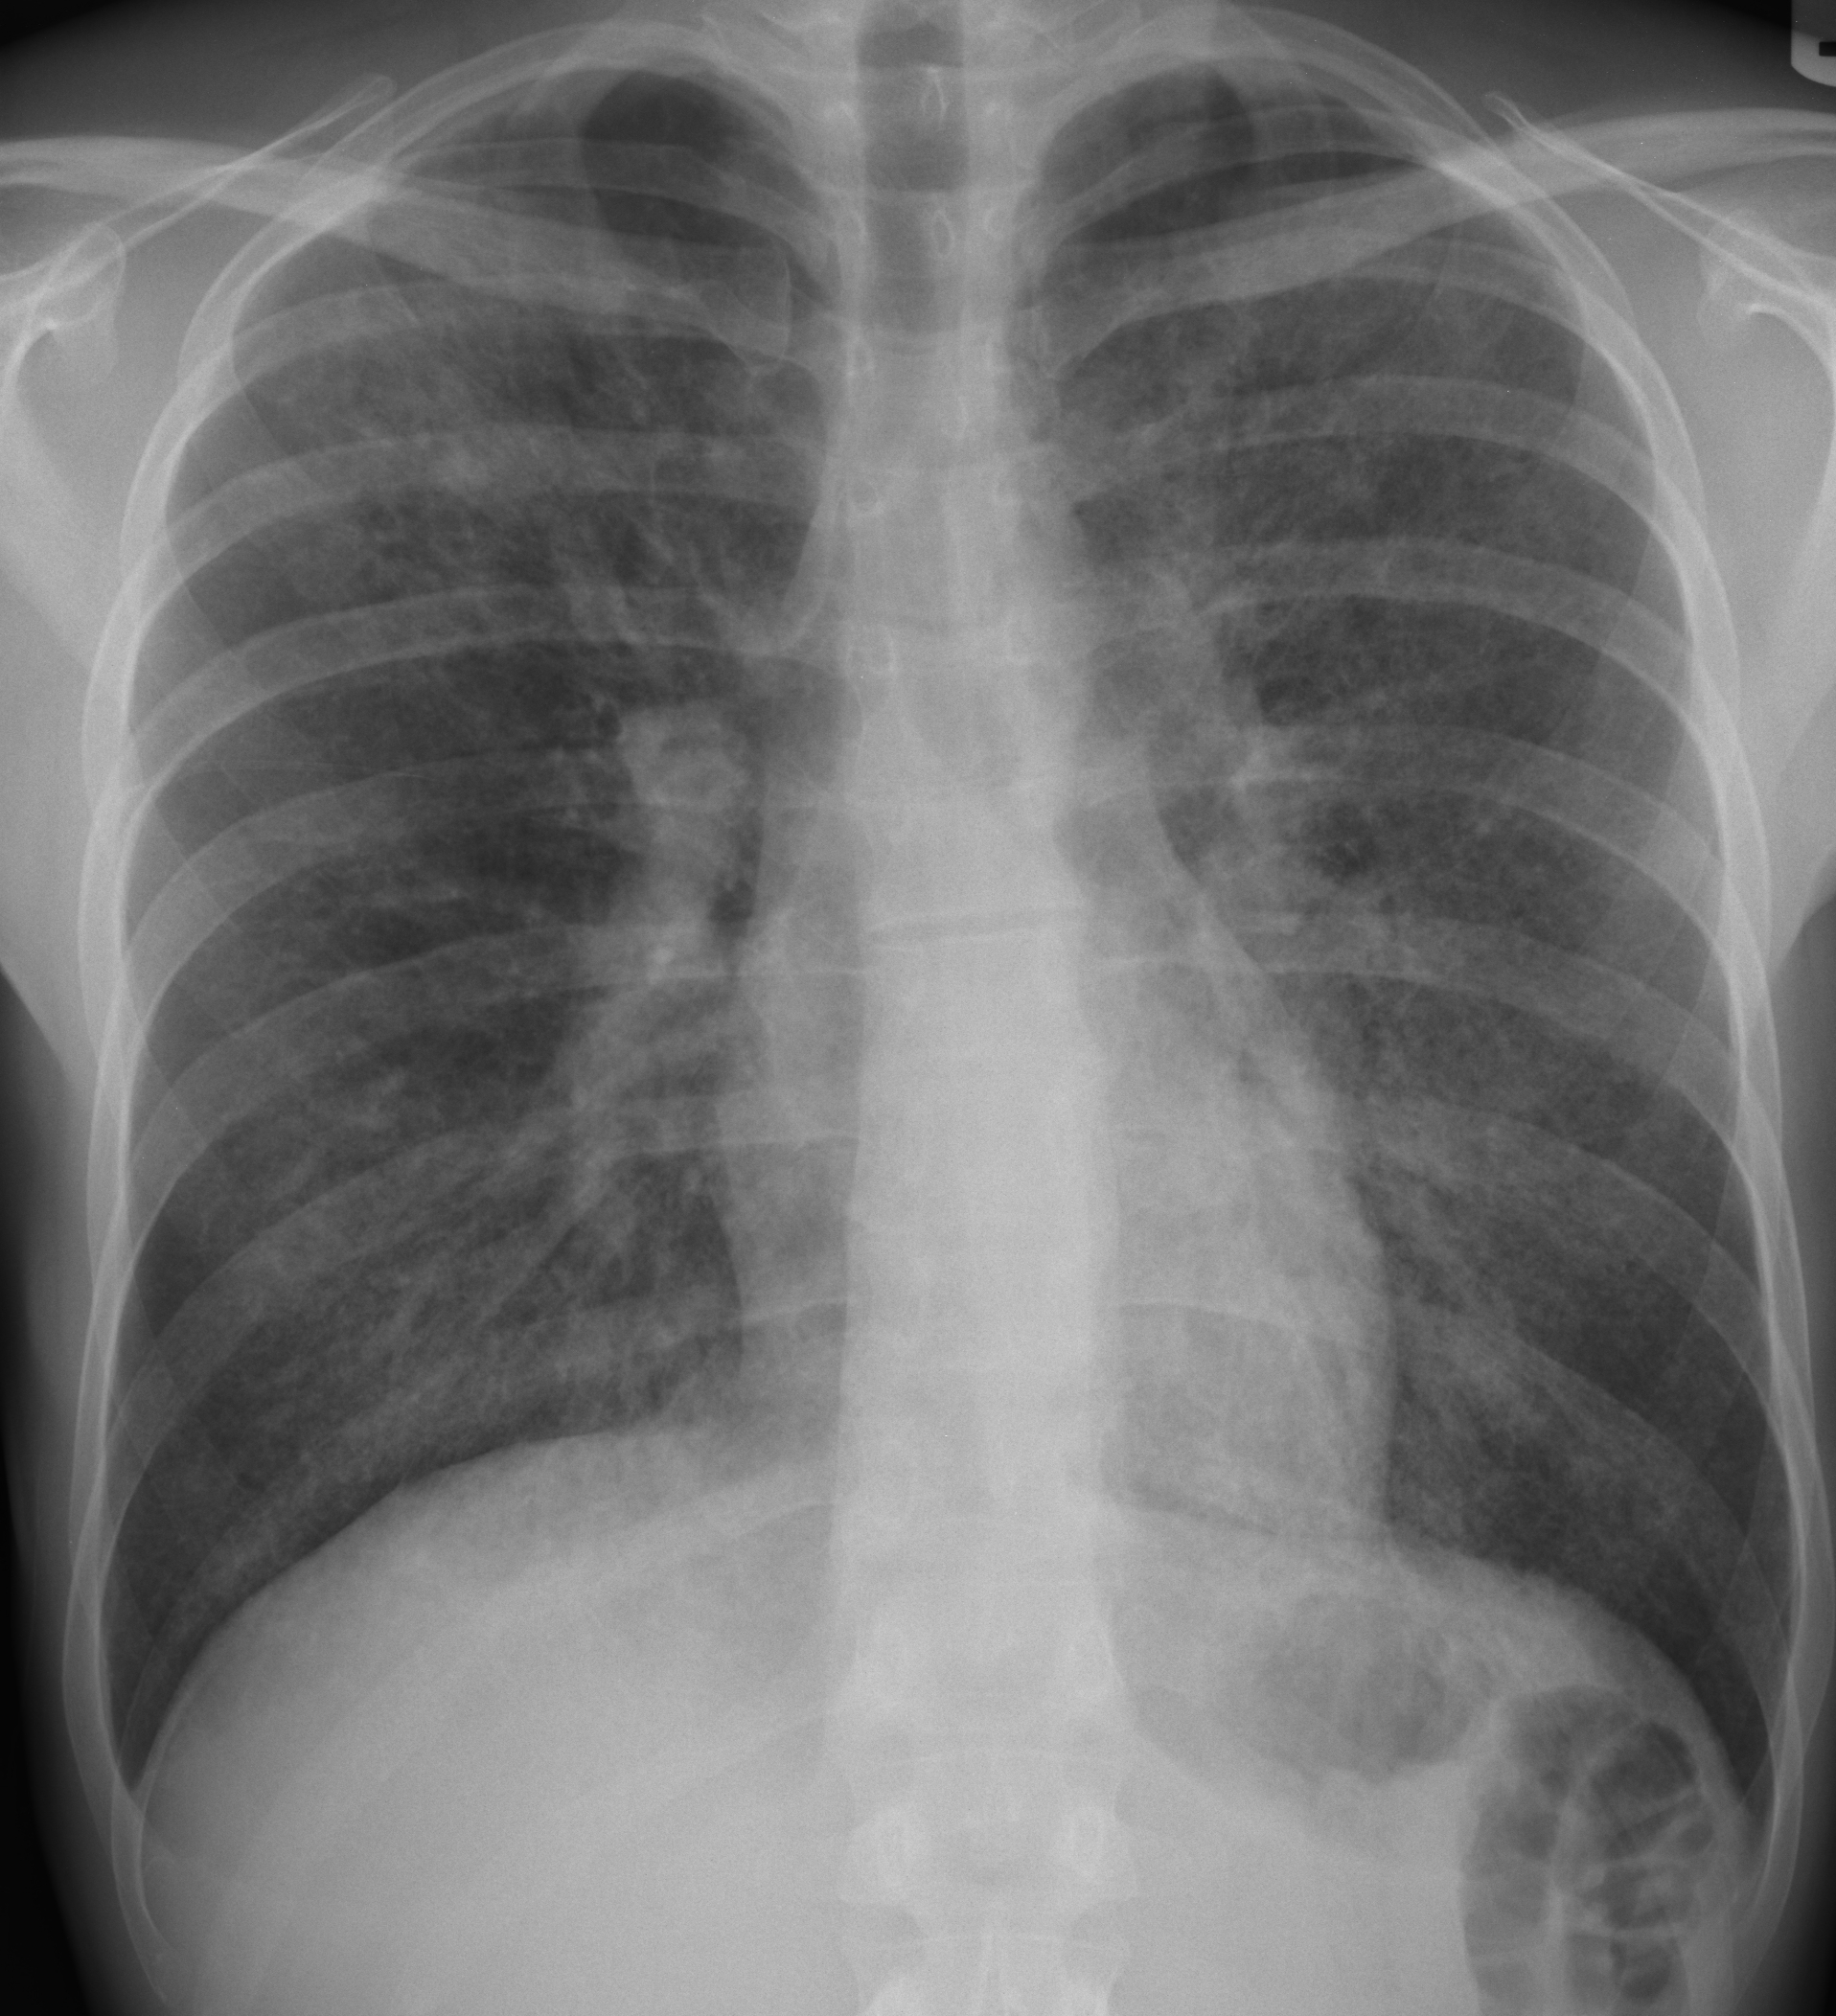
\includegraphics[height=3.6cm]{figures/healthcare_xray.jpg}}

\vspace{6pt}
\centerline{\textbf{Medical diagnosis}}
\centerline{pneumonia or healthy?}
\end{column}
\begin{column}{0.48\textwidth}
\centerline{%

\begin{tikzpicture}[
  mail/.style={draw, rounded corners, fill=gray!8, align=left,
    font=\small, text width=3.1cm, minimum height=1cm},
  tag/.style={font=\small\bfseries, text=white, rounded corners,
    inner sep=3pt}
]
  \node[mail] (m1) {\textbf{WIN a FREE prize!!!}\\ Click here now\dots};
  \node[mail, below=0.5cm of m1] (m2) {\textbf{Lab 2 moved}\\ Now on Thursday\dots};
  \node[tag, fill=red!70!black, below=0.08cm of m1.south east, anchor=north east] {spam};
  \node[tag, fill=green!50!black, below=0.08cm of m2.south east, anchor=north east] {not spam};
\end{tikzpicture}}

\vspace{6pt}
\centerline{\textbf{Spam filtering}}
\centerline{spam or not spam?}
\end{column}
\end{columns}

\vspace{10pt}
\begin{itemize}
\item[$\Rightarrow$] Same pattern in both: an input $\bs{x}$ (an X-ray,
  an email) $\mapsto$ a \textbf{discrete class label} $t$, here one of
  two classes.
\end{itemize}

\vspace{6pt}
{\scriptsize Image: chest X-ray showing \emph{Pneumocystis} pneumonia.
Samir, Wikimedia Commons, public domain.}

\end{frame}
%%%%%%%%%%%%%%%%%%%%%%%%%%%%%%%%%%%%%%%%%%%%%%%%%%%%%%%%%%%%%%%%%%%%%%
\begin{frame}[fragile]
\frametitle{Motivation: from a linear model to a probability}

\begin{itemize}
\item First instinct: reuse $y(\bs{x},\bs{w}) = \bs{w}^\top\bs\phi(\bs{x})$
  directly? Problem: it's unbounded, so it can't be read off as a
  probability, and doesn't respect $t\in\{0,1\}$.
\item[$\Rightarrow$] \textbf{Logistic regression}: squash the same linear
  function through a nonlinearity so its output is a valid probability.
\end{itemize}

\vspace{4pt}
\begin{columns}[T]
\begin{column}{0.5\textwidth}
\begin{itemize}
\item The \textbf{logistic sigmoid}:
\[
\sigma(a) = \frac{1}{1+e^{-a}}
\]
\item $\sigma(a) \to 0$ as $a\to-\infty$, $\sigma(a)\to1$ as
  $a\to+\infty$, $\sigma(0)=0.5$: output always in $(0,1)$.
\end{itemize}
\end{column}
\begin{column}{0.45\textwidth}
\resizebox{\linewidth}{!}{%
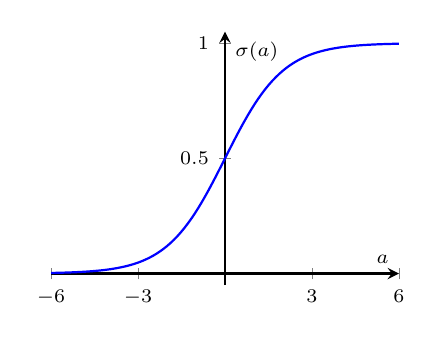
\begin{tikzpicture}
\begin{axis}[
  width=6cm, height=4.8cm,
  xlabel={$a$}, ylabel={$\sigma(a)$},
  xmin=-6, xmax=6, ymin=-0.05, ymax=1.05,
  xtick={-6,-3,0,3,6}, ytick={0,0.5,1},
  axis lines=middle,
  domain=-6:6, samples=100,
  thick,
  label style={font=\scriptsize},
  tick label style={font=\scriptsize},
]
\addplot[blue,thick] {1/(1+exp(-x))};
\end{axis}
\end{tikzpicture}}

\vspace{2pt}
{\scriptsize S-shaped: squashes any real $a$ into $(0,1)$.}
\end{column}
\end{columns}

\end{frame}
%%%%%%%%%%%%%%%%%%%%%%%%%%%%%%%%%%%%%%%%%%%%%%%%%%%%%%%%%%%%%%%%%%%%%%
\begin{frame}[fragile]
\frametitle{Logistic regression}

\begin{itemize}
\item Model the posterior probability of class $C_1$ as the
  \textbf{logistic sigmoid} applied to a linear function of the features $\bs\phi(\bs{x})$:
\[
p(C_1\mid\bs{x}) = y(\bs{x},\bs{w}) = \sigma\bigl(\bs{w}^\top\bs\phi(\bs{x})\bigr),
\qquad \sigma(a) = \frac{1}{1+e^{-a}}
\]
and $p(C_2\mid\bs{x}) = 1 - y(\bs{x},\bs{w})$.
% \item Only $M$ parameters $\bs{w}$, far fewer than modelling each class's
  % full distribution directly, especially as $M$ grows.
\end{itemize}

\begin{columns}[c]
\begin{column}{0.55\textwidth}
\centerline{\resizebox{\linewidth}{!}{%
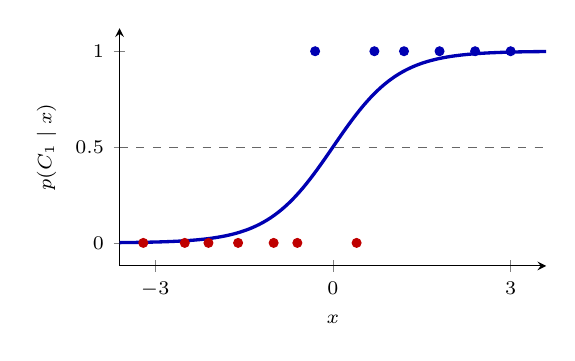
\begin{tikzpicture}
\begin{axis}[
  width=7cm, height=4.6cm,
  xlabel={$x$}, ylabel={$p(C_1\mid x)$},
  xmin=-3.6, xmax=3.6, ymin=-0.12, ymax=1.12,
  ytick={0,0.5,1}, xtick={-3,0,3},
  axis lines=left,
  label style={font=\scriptsize},
  tick label style={font=\scriptsize},
]
\addplot[black!60, dashed, domain=-3.6:3.6] {0.5};
\addplot[blue!70!black, very thick, domain=-3.6:3.6, samples=120] {1/(1+exp(-1.8*x))};
\addplot[only marks, mark=*, mark size=1.6pt, red!75!black]
  coordinates {(-3.2,0) (-2.5,0) (-2.1,0) (-1.6,0) (-1.0,0) (-0.6,0) (0.4,0)};
\addplot[only marks, mark=*, mark size=1.6pt, blue!70!black]
  coordinates {(-0.3,1) (0.7,1) (1.2,1) (1.8,1) (2.4,1) (3.0,1)};
\end{axis}
\end{tikzpicture}}}
\end{column}
\begin{column}{0.42\textwidth}
{\small
\begin{itemize}
\item 1-D example, $\bs\phi(x) = (1,x)^\top$: dots are the labels $t_n$
  ({\color{red!75!black}$C_2$} at 0, {\color{blue!70!black}$C_1$} at 1)
\item The fitted curve $\sigma(w_0 + w_1 x)$ gives a
  \emph{probability}, not a hard label
\item Near the overlap it is uncertain ($\approx 0.5$)
\end{itemize}}
\end{column}
\end{columns}

\end{frame}
%%%%%%%%%%%%%%%%%%%%%%%%%%%%%%%%%%%%%%%%%%%%%%%%%%%%%%%%%%%%%%%%%%%%%%
\begin{frame}[fragile]
\frametitle{Decision boundary}

\begin{columns}[T]
\begin{column}{0.53\textwidth}
\small
\begin{itemize}
\item Predict $C_1$ if $p(C_1\mid\bs{x}) > \theta$. Since $\sigma$ is
  monotonic, the boundary $p(C_1\mid\bs{x}) = \theta$ is
\[
\bs{w}^\top\bs\phi(\bs{x}) = \ln\frac{\theta}{1-\theta}
\]
\item $\theta = 0.5$ (equal cost for both mistakes, minimises error
  rate): $\bs{w}^\top\bs\phi(\bs{x}) = 0$
\item Other $\theta$ just \textbf{shift} the boundary parallel, e.g.\
  missing pneumonia is costly $\Rightarrow$ lower $\theta$, flag more
  patients
% \item Always \textbf{linear} in $\bs\phi$-space; with nonlinear basis
%   functions it can be curved in $\bs{x}$-space (next slide)
\end{itemize}
\end{column}
\begin{column}{0.44\textwidth}
\centerline{\resizebox{\linewidth}{!}{%
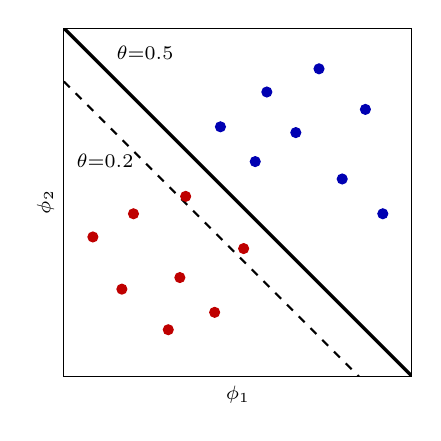
\begin{tikzpicture}
\begin{axis}[
  width=6cm, height=6cm,
  xlabel={$\phi_1$}, ylabel={$\phi_2$},
  xmin=-3, xmax=3, ymin=-3, ymax=3,
  xtick=\empty, ytick=\empty,
  axis lines=box,
  label style={font=\scriptsize},
]
\addplot[only marks, mark=*, mark size=1.8pt, blue!70!black] coordinates
  {(1,1.2) (1.8,0.4) (0.5,1.9) (2.2,1.6) (1.4,2.3) (0.3,0.7) (-0.3,1.3) (2.5,-0.2)};
\addplot[only marks, mark=*, mark size=1.8pt, red!75!black] coordinates
  {(-1,-1.3) (-1.8,-0.2) (-0.4,-1.9) (-2,-1.5) (-1.2,-2.2) (0.1,-0.8) (-0.9,0.1) (-2.5,-0.6)};
\addplot[black, very thick, domain=-3:3] {-x}
  node[pos=0.12, anchor=south west, font=\scriptsize] {$\theta{=}0.5$};
\addplot[black, thick, dashed, domain=-3:3] {-x-0.92};
\node[anchor=north west, font=\scriptsize] at (axis cs:-2.95,1.0) {$\theta{=}0.2$};
\end{axis}
\end{tikzpicture}}}

\vspace{2pt}
{\scriptsize Solid: $\theta{=}0.5$. Dashed: $\theta{=}0.2$, shifted towards
{\color{red!75!black}$C_2$}, so more points are labelled
{\color{blue!70!black}$C_1$}.}
\end{column}
\end{columns}

\vspace{4pt}
{\scriptsize See Bishop, \emph{PRML} (2006), Sections 1.5 and 4.3.2.}

\end{frame}
%%%%%%%%%%%%%%%%%%%%%%%%%%%%%%%%%%%%%%%%%%%%%%%%%%%%%%%%%%%%%%%%%%%%%%
\begin{frame}[fragile]
\frametitle{Linear in feature space, curved in input space}

\centerline{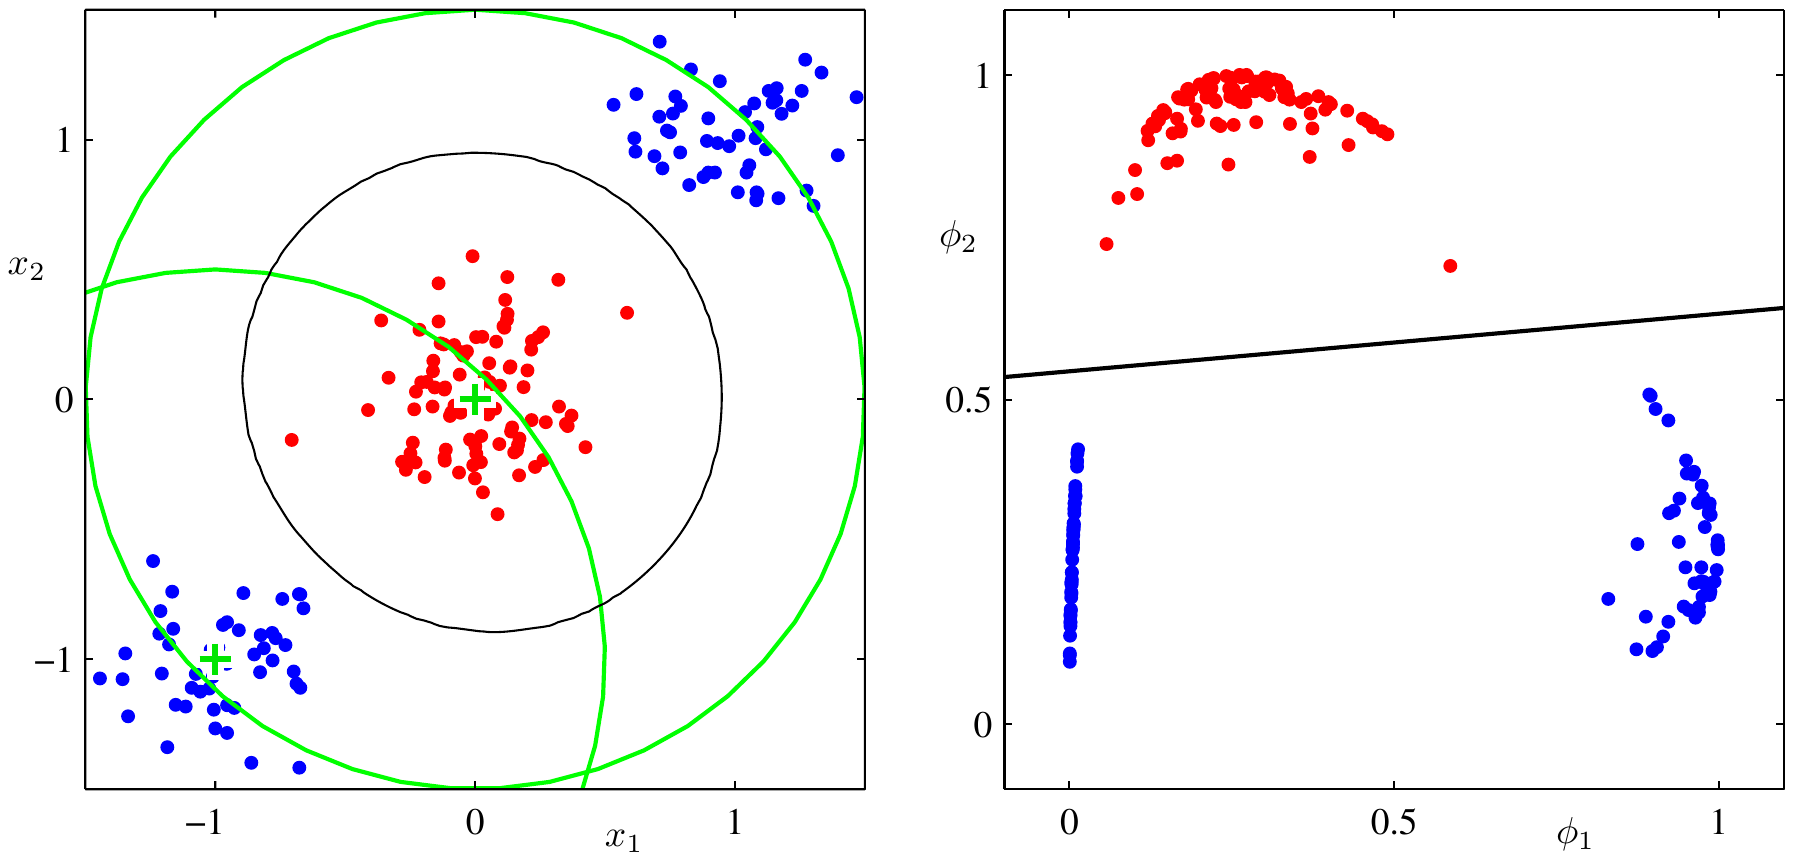
\includegraphics[width=0.8\textwidth]{figures/prml_fig4_12.png}}
\centerline{\hspace{0.9cm}{\small input space $\bs{x}$}\hspace{3.9cm}{\small
feature space $\bs\phi$}}

\vspace{4pt}
{\scriptsize Bishop, \emph{PRML} (2006), Fig.\ 4.12.}

\vspace{2pt}
\begin{itemize}
\small
\item Two Gaussian basis functions $\phi_1(\bs{x}),\phi_2(\bs{x})$
  (centres: green crosses) map each $\bs{x}$ to a point
  $(\phi_1,\phi_2)$.
\item Right: in $\bs\phi$-space a \textbf{straight line} separates the
  classes. Left: the same boundary, drawn in $\bs{x}$-space, is the
  black \textbf{circle}.
% \item[$\Rightarrow$] Good basis functions make linear models powerful;
%   neural networks \emph{learn} them from data (L04).
\end{itemize}

\end{frame}
%%%%%%%%%%%%%%%%%%%%%%%%%%%%%%%%%%%%%%%%%%%%%%%%%%%%%%%%%%%%%%%%%%%%%%
\begin{frame}[fragile]
\frametitle{Fitting logistic regression: the cross-entropy loss}

\begin{itemize}
\item With $t_n \in\{0,1\}$, the likelihood for a single point is
  \textbf{Bernoulli}:
\[
p(t_n\mid\bs{x}_n) = \begin{cases} y_n & t_n = 1\\ 1-y_n & t_n = 0
\end{cases}
\;=\; y_n^{t_n}(1-y_n)^{1-t_n}
\]
  with $y_n = \sigma(\bs{w}^\top\bs\phi_n) = p(C_1\mid\bs{x}_n)$ and
  $\bs\phi_n \equiv \bs\phi(\bs{x}_n)$: the exponents just switch
  between the two cases.
\item For the whole (i.i.d.) dataset, the likelihood is the
  \textbf{product}
\[
p(\bs{t}\mid\bs{w}) = \prod_{n=1}^{N} y_n^{t_n}(1-y_n)^{1-t_n}
\]
\item Taking $-\ln$ turns that product into a sum, the \textbf{cross-entropy
  loss function}:
\[
L(\bs{w}) = -\ln p(\bs{t}\mid\bs{w}) =
-\sum_{n=1}^{N}\bigl\{t_n \ln y_n + (1-t_n)\ln(1-y_n)\bigr\}
\]
\end{itemize}

\end{frame}
%%%%%%%%%%%%%%%%%%%%%%%%%%%%%%%%%%%%%%%%%%%%%%%%%%%%%%%%%%%%%%%%%%%%%%
\begin{frame}[fragile]
\frametitle{Fitting logistic regression: minimising the loss}

\begin{itemize}
\item The gradient of the cross-entropy loss is
\[
\nabla L(\bs{w}) = \sum_{n=1}^{N} (y_n - t_n)\, \bs\phi_n
\]
\emph{exactly the same form} as the least-squares gradient earlier,
with $y_n$ now the sigmoid output instead of $\bs{w}^\top\bs\phi_n$!
\end{itemize}

\vspace{6pt}
\begin{itemize}
\item[$\Rightarrow$] But $y_n$ is nonlinear in $\bs{w}$; no closed-form
  solution this time. Minimise $L(\bs{w})$ iteratively: gradient descent
  or SGD (end of this lecture), or Newton-Raphson (\emph{iteratively reweighted least
  squares}, Bishop \S4.3.3).
\end{itemize}

\end{frame}
%%%%%%%%%%%%%%%%%%%%%%%%%%%%%%%%%%%%%%%%%%%%%%%%%%%%%%%%%%%%%%%%%%%%%%
% \begin{frame}[fragile]
% \frametitle{Beyond two classes: softmax}

% \vfill
% \begin{columns}[c]
% \begin{column}{0.55\textwidth}
% \begin{itemize}
% \item For $K$ classes, use one score per class, $a_k =
%   \bs{w}_k^\top\bs\phi(\bs{x})$, and replace the sigmoid by the
%   \textbf{softmax}:
% \[
% p(C_k\mid\bs{x}) = \frac{\exp(a_k)}{\sum_{j=1}^{K}\exp(a_j)}
% \]
% \item For $K{=}2$ this reduces to the sigmoid.
% \end{itemize}
% \end{column}
% \begin{column}{0.42\textwidth}
% \centerline{\resizebox{\linewidth}{!}{%
% \begin{tikzpicture}
% \begin{axis}[
%   ybar, bar width=10pt,
%   width=5.4cm, height=4.4cm,
%   symbolic x coords={$C_1$,$C_2$,$C_3$},
%   xtick=data, ymin=0, ymax=2.5,
%   enlarge x limits=0.3,
%   legend style={font=\scriptsize, at={(0.98,0.98)}, anchor=north east},
%   tick label style={font=\scriptsize},
%   nodes near coords, every node near coord/.append style={font=\tiny},
% ]
% \addplot[fill=black!25] coordinates {($C_1$,2.0) ($C_2$,1.0) ($C_3$,0.1)};
% \addplot[fill=blue!55] coordinates {($C_1$,0.66) ($C_2$,0.24) ($C_3$,0.10)};
% \legend{score $a_k$, $p(C_k\mid\bs{x})$}
% \end{axis}
% \end{tikzpicture}}}

% \vspace{2pt}
% {\scriptsize Scores $(2.0, 1.0, 0.1)$ become probabilities
% $(0.66, 0.24, 0.10)$, summing to 1.}
% \end{column}
% \end{columns}

% \vspace{10pt}
% \begin{itemize}
% \item[$\Rightarrow$] Today we focus on $K{=}2$; see Bishop \S4.3.4 for
%   the multiclass details.
% \end{itemize}
% \vfill

% \end{frame}
%%%%%%%%%%%%%%%%%%%%%%%%%%%%%%%%%%%%%%%%%%%%%%%%%%%%%%%%%%%%%%%%%%%%%%
\begin{frame}[fragile]
\frametitle{Discuss: is 99\% accuracy good?}
\setbeamertemplate{blocks}[rounded]
\setbeamercolor{block title}{bg=orange!25,fg=black}
\setbeamercolor{block body}{bg=orange!7,fg=black}


\begin{block}{Discuss with your neighbour (1 min)}
A spam filter is tested on 1000 emails, of which only 10 are spam. It
labels \emph{every} email ``not spam'', so its accuracy is
$990/1000 = 99\%$.\\[3pt]
Is this a good filter? What is it missing?
\end{block}

\vspace{8pt}
\visible<2->{%
\begin{itemize}
\item It never catches a single spam email. Accuracy hides this, because
  ``not spam'' dominates the data (\textbf{class imbalance}).
\item[$\Rightarrow$] We need metrics that count each \emph{kind} of
  mistake separately: the \textbf{confusion matrix}.
\end{itemize}}

\end{frame}
%%%%%%%%%%%%%%%%%%%%%%%%%%%%%%%%%%%%%%%%%%%%%%%%%%%%%%%%%%%%%%%%%%%%%%
\begin{frame}[fragile]
\frametitle{How to evaluate a classification task: evaluation metrics}

\begin{columns}[c]
\begin{column}{0.44\textwidth}
\centerline{\resizebox{\linewidth}{!}{%
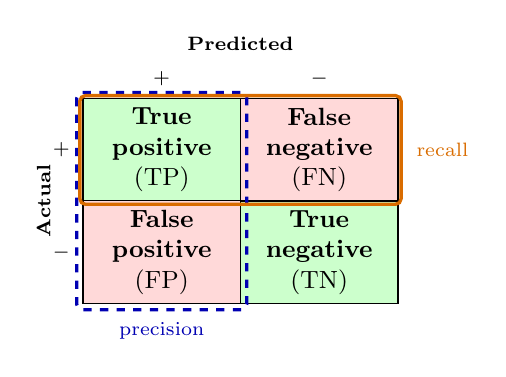
\begin{tikzpicture}[
  cell/.style={draw, minimum width=2cm, minimum height=1.3cm,
    align=center, font=\small},
  lab/.style={font=\scriptsize}
]
  \node[cell, fill=green!20] (tp) at (0,0)    {\textbf{True}\\\textbf{positive}\\(TP)};
  \node[cell, fill=red!15]   (fn) at (2,0)    {\textbf{False}\\\textbf{negative}\\(FN)};
  \node[cell, fill=red!15]   (fp) at (0,-1.3) {\textbf{False}\\\textbf{positive}\\(FP)};
  \node[cell, fill=green!20] (tn) at (2,-1.3) {\textbf{True}\\\textbf{negative}\\(TN)};
  \node[lab, above=1pt of tp] {$+$};
  \node[lab, above=1pt of fn] {$-$};
  \node[lab, left=1pt of tp] {$+$};
  \node[lab, left=1pt of fp] {$-$};
  \node[font=\scriptsize\bfseries] at (1,1.35) {Predicted};
  \node[font=\scriptsize\bfseries, rotate=90] at (-1.5,-0.65) {Actual};
  % precision: predicted-positive column; recall: actual-positive row
  \draw[blue!70!black, very thick, dashed, rounded corners=2pt]
    (-1.08,0.73) rectangle (1.08,-2.03);
  \draw[orange!85!black, very thick, rounded corners=2pt]
    (-1.04,0.69) rectangle (3.04,-0.69);
  \node[font=\scriptsize, text=blue!70!black, below=3pt of fp] {precision};
  \node[font=\scriptsize, text=orange!85!black, right=3pt of fn] {recall};
\end{tikzpicture}}}

\vspace{4pt}
{\scriptsize Positive ($+$) = the class we care about, e.g.\ spam or
pneumonia.}
\end{column}
\begin{column}{0.54\textwidth}
\small
\begin{itemize}
\item \textbf{Accuracy} $= \dfrac{\text{TP}+\text{TN}}{N}$:
  misleading when classes are imbalanced (previous slide)
\item {\color{blue!70!black}\textbf{Precision}} $=
  \dfrac{\text{TP}}{\text{TP}+\text{FP}}$: of the points
  \emph{predicted} positive, how many are actually positive?
\item {\color{orange!85!black}\textbf{Recall}} $=
  \dfrac{\text{TP}}{\text{TP}+\text{FN}}$: of the
  \emph{actually} positive points, how many did we catch?
\item \textbf{F1} $= \dfrac{2\cdot\text{Precision}\cdot
  \text{Recall}}{\text{Precision}+\text{Recall}}$: their
  harmonic mean, high only if both are
\end{itemize}
\end{column}
\end{columns}

\vspace{8pt}
\begin{itemize}
\item[$\Rightarrow$] As with regression, always evaluate on held-out
  (validation or test) data, not on the training set used to fit
  $\bs{w}$.
\end{itemize}

\end{frame}
%%%%%%%%%%%%%%%%%%%%%%%%%%%%%%%%%%%%%%%%%%%%%%%%%%%%%%%%%%%%%%%%%%%%%%
\begin{frame}[fragile]
\frametitle{A general view: loss functions}

\small
\begin{itemize}
\item Both regression and classification fit $\bs{w}$ the same way:
  choose a \textbf{loss function} $L(\bs{w})$ that measures how wrong
  the model's predictions are, then minimise it.
\item \textbf{Regression}: sum-of-squares loss
\[
L_D(\bs{w}) = \frac12 \sum_{n=1}^N \bigl\{t_n - y(\bs{x}_n,\bs{w})\bigr\}^2,
\qquad y_n = \bs{w}^\top\bs\phi_n
\]
\item \textbf{Classification}: cross-entropy loss
\[
L_D(\bs{w}) = -\sum_{n=1}^N \bigl\{t_n \ln y_n + (1-t_n)\ln(1-y_n)\bigr\},
\qquad y_n = \sigma(\bs{w}^\top\bs\phi_n)
\]
\end{itemize}

% \begin{itemize}
% \item Different tasks, different losses, but both gradients have the
%   \emph{same shape}:
% \[
% \nabla L(\bs{w}) = \sum_{n=1}^N (y_n - t_n)\, \bs\phi_n
% \]
% \end{itemize}

\begin{itemize}
\item Either can add a regularizer: $L(\bs{w}) = L_D(\bs{w}) +
  \lambda L_W(\bs{w})$ ($L_D$ = fit to the \emph{data}).
\item[$\Rightarrow$] A general pattern, not just these two: many other
  losses exist, e.g.\ absolute error (robust to outliers) or hinge loss
  (support vector machines). The right choice depends on the task; see
  the extension reading below.
\end{itemize}

\vspace{8pt}
{\footnotesize \textbf{Extension reading}, how to choose a loss for a
given task: Elharrouss et al., \emph{Loss Functions in Deep Learning: A
Comprehensive Review}, arXiv:2504.04242 (2025).
\href{https://arxiv.org/html/2504.04242v1}{\color{blue}arxiv.org/html/2504.04242v1}}

\end{frame}
%%%%%%%%%%%%%%%%%%%%%%%%%%%%%%%%%%%%%%%%%%%%%%%%%%%%%%%%%%%%%%%%%%%%%%
\begin{frame}[fragile]
\frametitle{Gradient descent}

\begin{columns}[c]
\begin{column}{0.53\textwidth}
\begin{itemize}
\item The normal equations invert the $M\times M$ matrix
  $\Phi^\top\Phi$: $O(M^3)$, costly for many features
\item Many losses (e.g.\ logistic regression's cross-entropy) have \emph{no}
  closed form
\item Instead, walk \textbf{downhill}: repeatedly step against the
  gradient,
\[
\bs{w}^{(\tau+1)} = \bs{w}^{(\tau)} - \eta\, \nabla L\bigl(\bs{w}^{(\tau)}\bigr)
\]
\end{itemize}
\end{column}
\begin{column}{0.44\textwidth}
\centerline{\resizebox{\linewidth}{!}{%
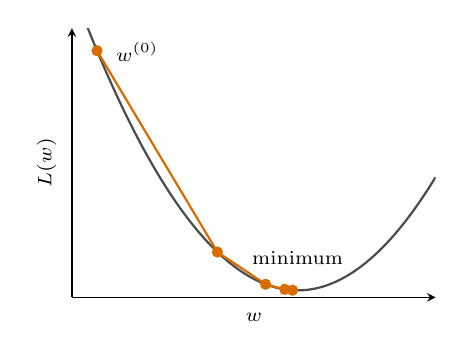
\begin{tikzpicture}
\begin{axis}[
  width=6.2cm, height=5cm,
  xlabel={$w$}, ylabel={$L(w)$},
  xmin=-2.6, xmax=3.2, ymin=0, ymax=11.5,
  xtick=\empty, ytick=\empty,
  axis lines=left,
  label style={font=\scriptsize},
]
\addplot[black!70, thick, domain=-2.6:3.2, samples=100] {(x-1)^2+0.3};
\addplot[orange!85!black, thick, -stealth, mark=*, mark size=1.6pt,
  mark options={fill=orange!85!black}] coordinates {(-2.200,10.540) (-0.280,1.938) (0.488,0.562) (0.795,0.342) (0.918,0.307)};
\node[font=\scriptsize, anchor=west] at (axis cs:-2.05,10.5) {$w^{(0)}$};
\node[font=\scriptsize, anchor=south] at (axis cs:1,1.0) {minimum};
\end{axis}
\end{tikzpicture}}}

\vspace{2pt}
{\scriptsize Each step moves downhill; steps shrink as the slope
flattens near the minimum.}
\end{column}
\end{columns}

\end{frame}
%%%%%%%%%%%%%%%%%%%%%%%%%%%%%%%%%%%%%%%%%%%%%%%%%%%%%%%%%%%%%%%%%%%%%%
\begin{frame}[fragile]
\frametitle{Gradient descent: learning rate and cost}

\begin{itemize}
\item $\eta$ = \textbf{learning rate}: too small $\Rightarrow$ slow;
  too large $\Rightarrow$ overshoots and can diverge.
\end{itemize}

\centerline{%
\resizebox{0.45\textwidth}{!}{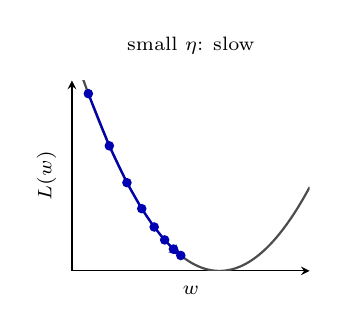
\begin{tikzpicture}
\begin{axis}[
  width=4.6cm, height=4cm, title={\scriptsize small $\eta$: slow},
  xlabel={$w$}, ylabel={$L(w)$},
  xmin=-2.6, xmax=3.2, ymin=0, ymax=11,
  xtick=\empty, ytick=\empty, axis lines=left,
  label style={font=\scriptsize},
]
\addplot[black!70, thick, domain=-2.6:3.2, samples=100] {(x-1)^2};
\addplot[blue!70!black, thick, -stealth, mark=*, mark size=1.3pt,
  mark options={fill=blue!70!black}] coordinates {(-2.200,10.240) (-1.688,7.225) (-1.258,5.098) (-0.897,3.597) (-0.593,2.538) (-0.338,1.791) (-0.124,1.264) (0.056,0.892)};
\end{axis}
\end{tikzpicture}}
\hspace{0.4cm}
\resizebox{0.45\textwidth}{!}{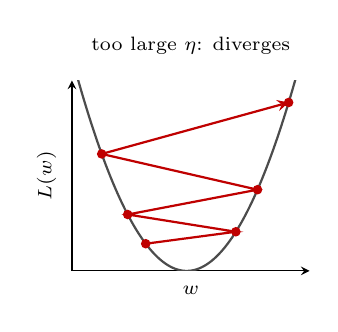
\begin{tikzpicture}
\begin{axis}[
  width=4.6cm, height=4cm, title={\scriptsize too large $\eta$: diverges},
  xlabel={$w$}, ylabel={$L(w)$},
  xmin=-1.8, xmax=4.0, ymin=0, ymax=7,
  xtick=\empty, ytick=\empty, axis lines=left,
  label style={font=\scriptsize},
]
\addplot[black!70, thick, domain=-1.8:4.0, samples=100] {(x-1)^2};
\addplot[red!75!black, thick, -stealth, mark=*, mark size=1.3pt,
  mark options={fill=red!75!black}] coordinates {(0.000,1.000) (2.200,1.440) (-0.440,2.074) (2.728,2.986) (-1.074,4.300) (3.488,6.192)};
\end{axis}
\end{tikzpicture}}}

\vspace{6pt}
\begin{itemize}
\item[$\Rightarrow$] \textbf{Batch} GD, $\nabla L(\bs{w}) = \sum_{n=1}^N
  \nabla L_n(\bs{w})$, still touches all $N$ points at \emph{every}
  step: costly for large $N$ $\Rightarrow$ SGD (next).
\end{itemize}

\end{frame}
%%%%%%%%%%%%%%%%%%%%%%%%%%%%%%%%%%%%%%%%%%%%%%%%%%%%%%%%%%%%%%%%%%%%%%
\begin{frame}[fragile]
\frametitle{Stochastic gradient descent (SGD)}

\begin{columns}[c]
\begin{column}{0.54\textwidth}
\small
\begin{itemize}
\item \textbf{Stochastic} (online): use the gradient of a
  \emph{single} point's loss $L_n(\bs{w})$ per step:
\[
\bs{w}^{(\tau+1)} = \bs{w}^{(\tau)} - \eta\, \nabla L_n\bigl(\bs{w}^{(\tau)}\bigr)
\]
\item Least squares, $L_n = \frac12(t_n - \bs{w}^\top\bs\phi_n)^2$:
  $\nabla L_n(\bs{w}) = (\bs{w}^\top\bs\phi_n - t_n)\,\bs\phi_n$, the
  \textbf{least-mean-squares} (LMS) algorithm.
\item Logistic regression: the same update, with $y_n =
  \sigma(\bs{w}^\top\bs\phi_n)$ in place of $\bs{w}^\top\bs\phi_n$.
\end{itemize}
\end{column}
\begin{column}{0.43\textwidth}
\centerline{\resizebox{\linewidth}{!}{%
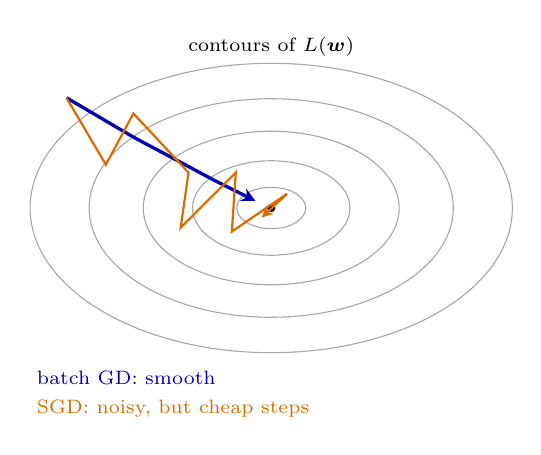
\begin{tikzpicture}
  \foreach \r in {0.35,0.8,1.3,1.85,2.45}
    \draw[black!35] (0,0) ellipse ({1.25*\r} and {0.75*\r});
  \fill (0,0) circle (1.5pt);
  \draw[blue!70!black, very thick, -stealth]
    (-2.6,1.4) -- (-1.75,0.9) -- (-1.15,0.58) -- (-0.72,0.35)
    -- (-0.42,0.2) -- (-0.2,0.09);
  \draw[orange!85!black, thick, -stealth]
    (-2.6,1.4) -- (-2.1,0.55) -- (-1.75,1.2) -- (-1.05,0.45)
    -- (-1.15,-0.25) -- (-0.45,0.45) -- (-0.5,-0.3) -- (0.2,0.18)
    -- (-0.12,-0.12);
  \node[font=\scriptsize, text=blue!70!black, anchor=west] at (-3.1,-2.15)
    {batch GD: smooth};
  \node[font=\scriptsize, text=orange!85!black, anchor=west] at (-3.1,-2.55)
    {SGD: noisy, but cheap steps};
  \node[font=\scriptsize] at (0,2.05) {contours of $L(\bs{w})$};
\end{tikzpicture}}}
\end{column}
\end{columns}

\vspace{6pt}
\begin{itemize}
\item[$\Rightarrow$] Scales to huge/streaming datasets (no
  $\Phi^\top\Phi$, no full-batch gradient); the same idea trains neural
  networks (L04).
\end{itemize}

\vspace{2pt}
{\scriptsize See Bishop, \emph{PRML} (2006), Section 3.1.3.}

\end{frame}
%%%%%%%%%%%%%%%%%%%%%%%%%%%%%%%%%%%%%%%%%%%%%%%%%%%%%%%%%%%%%%%%%%%%%%
\begin{frame}[fragile]
\frametitle{SGD: the algorithm}

\centerline{\begin{minipage}{0.8\textwidth}
\begin{algorithm}[H]
\DontPrintSemicolon
\KwIn{learning rate $\eta$, initial weights $\bs{w}$}
\Repeat{validation loss stops improving, or max epochs reached}{
  shuffle the $N$ training points\;
  \For{$n = 1,\dots,N$}{
    $\bs{w} \leftarrow \bs{w} - \eta\, \nabla L_n(\bs{w})$\;
  }
}
\end{algorithm}
\end{minipage}}

\vspace{8pt}
\begin{itemize}
\item One pass through all $N$ points is one \textbf{epoch}.
\item \textbf{Shuffle} each epoch, so the updates don't follow the same
  fixed order every time.
\item \textbf{When to stop}: after a fixed number of epochs, or when the
  loss on a held-out \emph{validation} set stops improving.
\end{itemize}

\end{frame}
%%%%%%%%%%%%%%%%%%%%%%%%%%%%%%%%%%%%%%%%%%%%%%%%%%%%%%%%%%%%%%%%%%%%%%
\begin{frame}[fragile]
\frametitle{Summary}

\vfill
\begin{itemize}
\item \textbf{Least squares} $=$ maximum likelihood under Gaussian noise
\vspace{4pt}
\item \textbf{Regularization} $\lambda L_W(\bs{w})$ curbs overfitting
\vspace{4pt}
\item \textbf{Logistic regression}: $\sigma(\bs{w}^\top\bs\phi(\bs{x}))$, cross-entropy loss
\vspace{4pt}
\item \textbf{Evaluation}: confusion matrix, precision, recall, F1
\vspace{4pt}
\item \textbf{(S)GD}: minimise any loss iteratively, scales to large $N$
\vspace{4pt}
% \item[$\Rightarrow$] Next (L04): neural networks learn the basis functions
\end{itemize}
\vfill

\end{frame}
%%%%%%%%%%%%%%%%%%%%%%%%%%%%%%%%%%%%%%%%%%%%%%%%%%%%%%%%%%%%%%%%%%%%%%
\begin{titledslide}{Reading}

  \begin{itemize}
  \item Bishop, C.\,M., \emph{Pattern Recognition and Machine Learning}
    (2006).
    \href{https://www.microsoft.com/en-us/research/uploads/prod/2006/01/Bishop-Pattern-Recognition-and-Machine-Learning-2006.pdf}{Free
      online}.
  % \item Today's material:
    \begin{itemize}
    \item Chapter 1: \S1.1 (overfitting), \S1.2.5 (probabilistic view),
      \S1.5 (decision thresholds)
    \item Chapter 3: \S3.1 (maximum likelihood, sequential learning,
      regularization, multiple outputs)
    \item Chapter 4: \S4.3.1--4.3.2 (fixed basis functions, logistic
      regression)
    \end{itemize}
  % \item Extension reading: Elharrouss et al., \emph{Loss Functions in
  %   Deep Learning: A Comprehensive Review}, arXiv:2504.04242 (2025).
  %   \href{https://arxiv.org/html/2504.04242v1}{Link}.
  % \item Same notation as last lecture, except inputs are now vectors
  %   $\bs{x}$: targets $t$, basis functions $\bs\phi(\bs{x})$, weights $\bs{w}$.
  \end{itemize}

\end{titledslide}
%%%%%%%%%%%%%%%%%%%%%%%%%%%%%%%%%%%%%%%%%%%%%%%%%%%%%%%%%%%%%%%%%%%%%%
\end{document}
